\documentclass[a4paper,12pt]{article}
%\usepackage[ngerman]{babel}
\usepackage{ucs}
\usepackage{multirow}
\usepackage{xltxtra}
\usepackage[utf8x]{inputenc}
\usepackage{fontspec}
\usepackage[automark]{scrpage2}
\usepackage{eurosym}
\usepackage{graphicx}
\usepackage[paper=a4paper,left=25mm,right=25mm,top=25mm,bottom=25mm]{geometry}
\pagestyle{scrheadings}
\setmainfont[Mapping=tex-text]{Liberation Serif}
\clearscrheadfoot
\begin{document}
\ohead{Last edit: \today}
\title{Rules Fire Fighting Challenge 2018}

 \begin{center}

\includegraphics[width=0.5\textwidth]{logo.png}

\huge                      % Schriftgröße einstellen
\bfseries                   % Fettdruck einschalten
Rules Fire Fighting Challenge 2018
  \end{center}
  This is only an unofficial translation. In case of any doubt, only the newest official version of the German rules will
  count. Changes in the rules since 2017 are marked in \textbf{bold}.
\section{Goal}
To design, build, and program a robot that can locate and extinguish 4 randomly placed candles inside a field
described by a black line. The first candle is in plain view of the starting position of the robot, the remaining
three candles are obstructed by walls. The faster you can extinguish the 4 candles increases your overall
score.
\section{Who Can Play}
Teams of \emph{2 to 4 players} in \emph{separate divisions} for:
\begin{itemize}
	\item Middle School (Age 10-13)
	\item High School (Age 14-17)
	\item Big Kids (Age 18-20)
\end{itemize}
\section{Required Materials}
Autonomous robot, any platform, costing €1,500 EUR or less, and meets the following design constraints,
which will be verified during Check-In:
\begin{itemize}
\item Robot can demonstrate it is running a program that can control the start and stop of its extinguishing system
via a sensor that interacts with either the candle or the circle the candle is placed on.
\item If using a high speed propeller, you must ensure that nobody can be injured by the propeller.
\item Volume of the robot must not exceed 65030 cubic cm. Multiple sensors and processors are allowed.
\end{itemize}
\section{Challenge Specifications}
\begin{itemize}
\item Challenge field is approximately 2.4 m by 3.6 m.
\item A border will be constructed using white and black duct tape.
\item The border’s white duct tape will be 7.5 cm wide with a 2.5 cm black duct tape line
down the center of the white tape.
\item Candles and walls will be randomly placed for every run.
\item The candles stand at the center of a white vinyl circle, ~ 40.5 cm diameter, and has
a 2.5 cm black line that is 2.5 cm inside the outer edge. The circle has a 5 cm
diameter black circle at its center to indicate where the candle will be placed.
\item The height of the candle is 25.5cm (from the ground to the bottom of the flame) 3
candles are covered by one wall each. 1 candle is visible from the starting location
of the robot.
\item The walls are 46 cm wide and 43 cm tall. They are held up by wooden bases that
are 3.5 cm tall and span the entire width of the wall.
sichtbar
\item The Challenge is run in an area that has a skylight above it. As the day progresses the sun changes position
and the sunlight from above is constantly changing in both position and brightness. Be prepared to engineer
around this natural condition.
\end{itemize}
\begin{center}
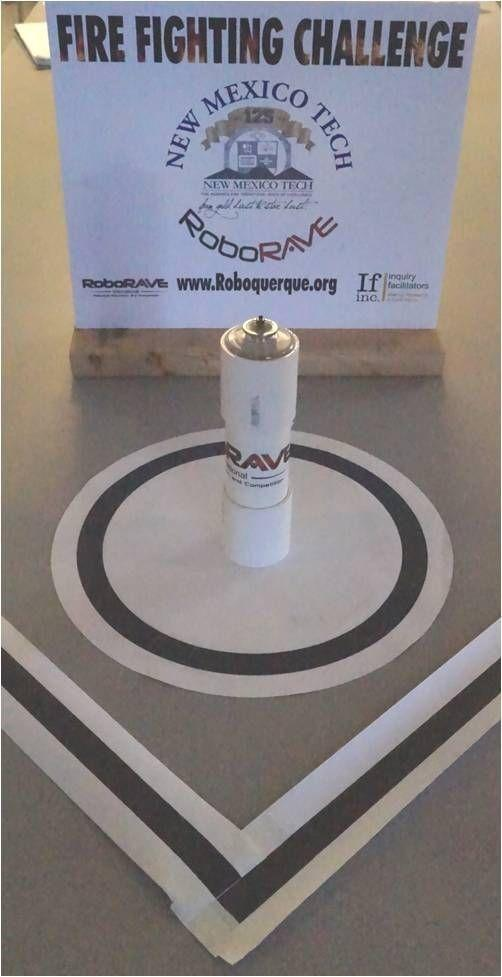
\includegraphics[width=0.4\textwidth]{candle.jpeg}
\end{center}
\section{General Rules of Play}
\begin{itemize}
	\item Robot will start the challenge at a spot on the border chosen by the Challenge Oficial.
	\item The first candle will be in plain view of the robot at the start of the challenge.
	\item The robot has 3 minutes to extinguish the 4 candles.
	\item Only players can operate and manipulate the robot during the heat (Players play, Coaches Coach).
	\item If a player touches the robot after the challenge has begun, the time stops, the run ends, and the challenge will
	be scored based on the number of candles extinguished when the robot was touched.
\end{itemize}
\section{Scoring Period}
\par The way the earned points are counted for the challenge will be announced on the first day of the event.
\section{Scoring}
The overall score is a combination of points earned during the challenge attempt added to the number of
seconds remaining once the last candle is extinguished. Therefore it is possible to achieve 100 regular points and 180 bonus points fpr time.
\section{Penalty Rules}
\begin{itemize}
\item Robot’s extinguishing system is engaged before any part of robot is over the white circle. \textbf{(No points for this candle)}
\item \textbf{If a candle is extinguished before the robot is over the white circle the number points for the following candle will not be increased.}
\item Robot touches the candle in the process of extinguishing the flame. The process of
extinguishing the
candle is not complete until the flame is out, and all the parts of the robot are no longer over the white
circle. (only 50\% of points for this candle)
\item Previously extinguished candles become obstacles in the playfield, and do not count as a penalty when
touched.
\end{itemize}
\section{Scoring matrix}
\begin{center}
\begin{tabular}{|c|c|c|c|c|c|} \hline
	 & 1. Candle & 2. Candle & 3. Candle & 4. Candle  \\ \hline
	 Outside circle & - & - & - & - \\ \hline
	Robot touches candle & 50 & 100 & 150 & 200 \\ \hline
Full Points & 100 & 200 & 300 & 400  \\ \hline
\end{tabular}
\end{center}
\end{document}